\section*{5/22}
  \underline{Example}: Random walk on the graph: The walker chooses a neighbor at 
    random, then moves there. What is the proportion of time spent at 0.

  \subsection*{Reversible Markov Chain}
    Assume that a chain starts in the invariant distribution, $X_0, X_1, \ldots,
    X_n$ has the same statistics on the time-reversal as $X_n, X_{n-1}, \ldots,
    X_0$, then we call the chain \underline{reversible}.
    Formally, we can define such chains as follows:
    $$
      P(X_{m} = j | X_{m-1} = i) = P(X_{m-1} = j | X_m = i)
    $$
    Moving forwards = Moving backwards.\\

    Let $\pi_i$ be the invariant distribution and let $\pi_i$ be the initial
    distribution, then equation says that $P_{ij} = \frac{P(X_{m-1}) = j, 
    X_m = i}{P(X_m = i)} = P(X_{m-1} = j) P(X_{m} = i | X_{m - 1} = j) = 
    \frac{\pi_jP_{ji}}{\pi_i}$.\\

    A Markov Chain is reversible with respect to invariant distribution $\pi_i$
    when $\pi_i P_{ij} = \pi_j P_{ji}$.\\

    \begin{proposition}
    If a probability mass function, $\pi_i$ satisfies
    $\pi_iP_{ij} = \pi_jP_{ji}$, then it is automatically invariant.
    \end{proposition}
    \begin{proof}
      Need to check $\pi_j = \sum_i \pi_i P_{ij}$.\\
      We know that $\sum_i \pi_i P_{ij} = \sum_i \pi_j P{ji}
      = \pi_j \sum_{i}^n P_{ji} = \pi_j D$\\
      More general problem: Assign nonnegative weights to any edge in
      a complete graph, $w_{ij} = w_{ji}$ is the weight of the edge
      between $i$ and $j$.\\
      When in $i$, the walker goes to $j$ with probability 
      proportional to $w_{ij}$, so $P_{ij} = \frac{w_{ij}}{\sum_j
      w_{ij}}$.\\
      $$
        \pi_i = \frac{\sum_j w_{ij}}{\sum_{i,j} w_{ij}}
      $$
      is a reversible measure. why? $\pi_i P_{ij} = \pi_j P_{ji}$.
      This is equivalent to $\sum_j w_{ij} \frac{w_{ij}}{\sum_j 
      w_{ij}} = \sum_i w_{ij} \frac{w_{ij}}{\sum_i w_{ij}}$.\\
    \end{proof}
    \underline{Remark}: This chain is irreducible exactly when the
      graph with edge\{$i$, $j$\} whenever $w_{ij} > 0$ is connected.
      Aperiodic $\Leftrightarrow$ not bipartite.\\

    \noindent \underline{Example}: Back to the walker problem.\\
      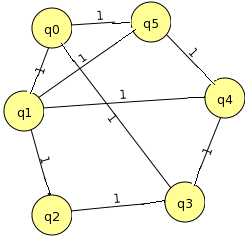
\includegraphics[height=50mm]{figure_9.png}\\
      \begin{eqnarray*}
        \pi_0 & = & \frac{3}{18}\\
        \pi_1 & = & \frac{3}{18}\\
        \pi_2 & = & \frac{3}{18}\\
        \pi_3 & = & \frac{3}{18}\\
        \pi_4 & = & \frac{3}{18}\\
        \pi_5 & = & \frac{3}{18}\\
      \end{eqnarray*}
      Therefore, proportion of time spent at 0 is $\frac{1}{6}$.\\
      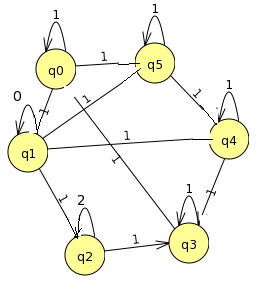
\includegraphics[height=60mm]{figure_10.png}\\

    \noindent \underline{Example}: Ehrenfest chain\\
      $M$ balls, two urns. Each time, pick a ball at random, move it from one urn to
      another.\\
      Let $X_n$ be the number of balls in urn 1.\\
      \begin{eqnarray*}
        P_{0, 1} & = & 1\\
        P_{M, M - 1} & = & 1\\
        P_{i, i - 1} & = & \frac{i}{M}\\
        P_{i, i + 1} & = & \frac{M - i}{M}\\
      \end{eqnarray*}
      With some intuitive guessing, you can see $\pi_i = \binom{M}{i}\frac{1}{2^M}$.\\
      Let's prove this. First, check for reversibility. Are the following true?
      \begin{eqnarray*}
        \pi_0 P_{01} & = & \pi_1 P_{10}\\
        \pi_i P_{i, i+1} & = & \pi_{i + 1} P_{i + 1, i}\\
        \pi_i P_{i, i-1} & = & \pi_{i - 1} P_{i - 1, i}\\
        \pi_M P_{M, M-1} & = & \pi_{M - 1} P_{M - 1, i}\\
      \end{eqnarray*}
      For the first equation
      \begin{eqnarray*}
        \pi_0 P_{01} & = & \pi_1 P_{10}\\
        \frac{1}{2^M} \cdot 1 & = & M \frac{1}{2^M} \cdot \frac{1}{M}\\
        1 & = & 1
      \end{eqnarray*}
      You can check the other equations, it matches.\\
      Also, note that this chain is irreducible, but not aperiodic. It has period 2.
